%\subsection{SLOSH}
Storm surge, measured as water height above ground level, can produce flooding as a result
    of a storm pushing sea-water onto land.  Its effects can be catastrophic, potentially
    disrupting critical infrastructure such as emergency services, logistical services,
    and military responsiveness.   The Sea, Lake, and Overland Surges from Hurricanes 
    (SLOSH)\citep{jelesnianski1992} is a 
    computer model developed by the National Weather Service to simulate storm 
    surge, and its associated inundation caused by hurricanes.   Given storm 
    characteristics, the model takes into account local topology, bathymetry, 
    and surge management devices such as levees, to generate a spatial field of 
    inundation---the maximum observed height of water above ground level 
    (or above normal water level for a data point in a body of water) over the 
    duration of the storm at a location.   These storm characteristics are
    data pertaining to the eye of the storm when it made landfall---bearing, 
    velocity, latitude, minimum atmospheric pressure of the storm when it 
    made landfall, and projections of sea level rise over time.  The example that motivates
    this work corresponds to a \emph{simulation} from SLOSH, covering an area extending 
    from Virginia Beach, Virginia, to Long Island, New York.
    The simulation output describes the surge over a grid containing some \num{23119800} 
    elements, with a spatial resolution of \num{0.001} degrees, or approximately 90 
    meters.   We have \num{4000} such simulations, produced from a sample of 
    storm characteristics.

% \begin{figure}[t!]
%     \centering
%     \begin{subfigure}[t]{0.48\textwidth}
%         \centering
%         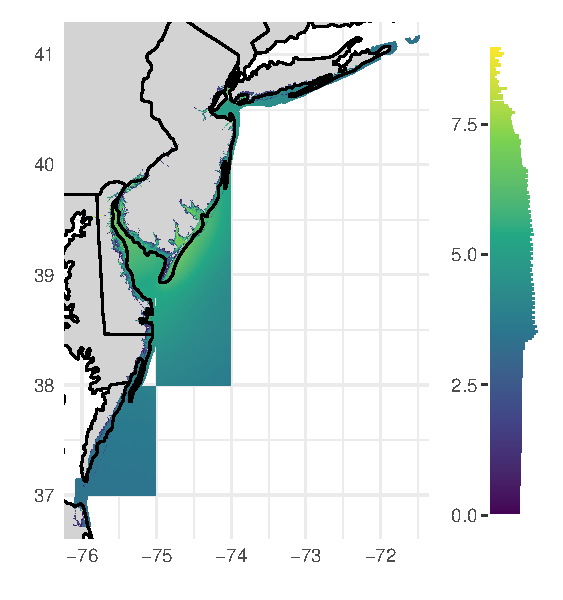
\includegraphics[width=0.99\linewidth]{./plots/slosh1run_loghist.pdf}
%         \caption{Grid output from one storm simulation in SLOSH, with a marginal
%             histogram (with log-scale counts) of surge levels in that storm 
%             (truncated at 9 feet).\label{fig:slosh1run}\makenote{add boundaries to indicate
%             range of directions and latitudes at which storm makes landfall.}}
%     \end{subfigure}%
%     ~ 
%     \begin{subfigure}[t]{0.48\textwidth}
%         \centering
%         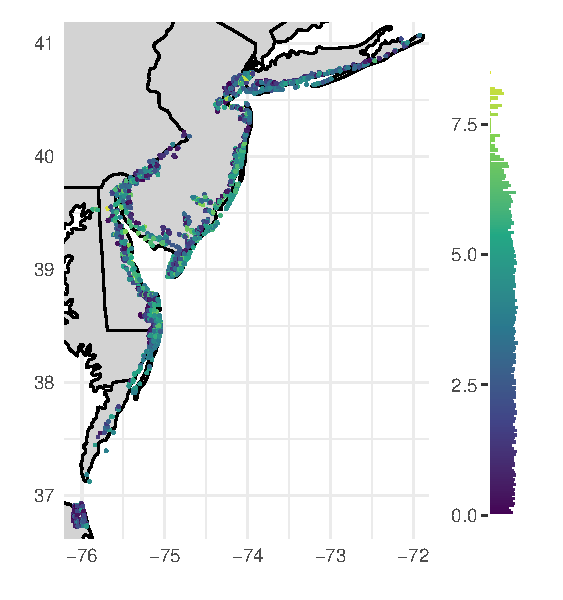
\includegraphics[width=0.99\linewidth]{./plots/sloshthreshold_loghist.pdf}
%         \caption{
%             90th percentile of storm-surge simulations at \num{5283} selected 
%             locations with marginal histogram (with log-scale counts).
%             \label{fig:sloshthreshold}}
%     \end{subfigure}
%     \caption{Exploration of SLOSH simulation data.\label{fig:sloshexplore}}
% \end{figure}

\begin{figure}[t!]
    \centering
    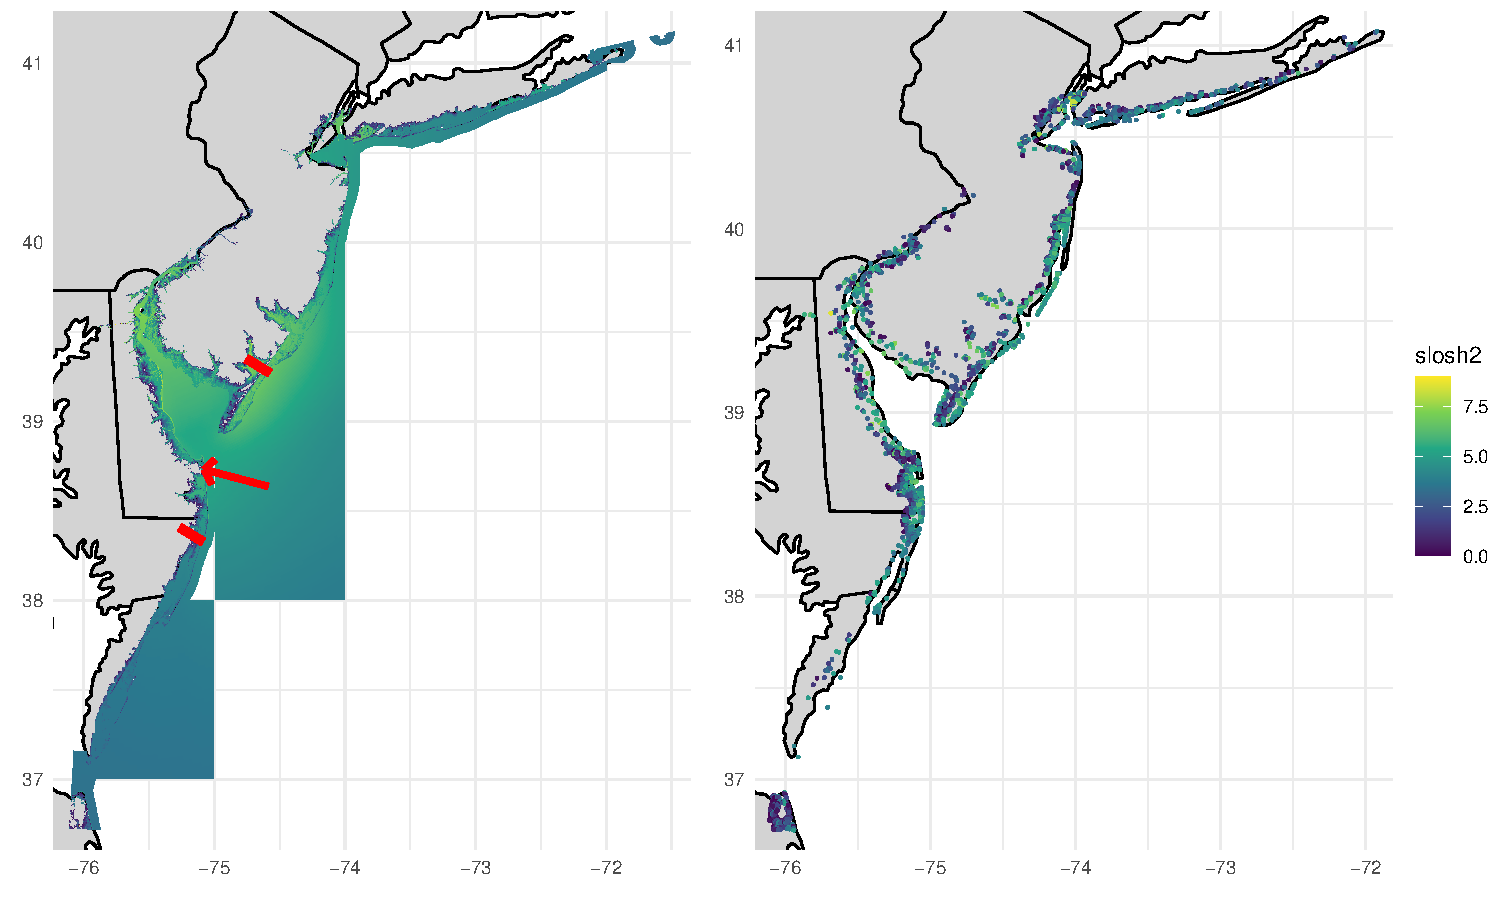
\includegraphics[width = 0.8\linewidth]{./plots/slosh_combined}
    \caption{(Left) Grid output from one storm simulation in SLOSH, with values 
    truncated at 9 feet.  The bars (red) indicate the lower and upper limits on the 
    location of the hurricane eye at landfall.  The arrow indicates the direction 
    of travel, and at the vertex, the location of the hurricane eye at landfall 
    for this realization of the SLOSH output grid.  (Right) Marginal 90th 
    percentiles of simulated storm-surge at selected locations within the grid. 
    \label{fig:sloshexplore}\makenote{Remove legend name, or rename to `Surge'.
    Increase legend height to match that of maps.  Make thinner, if possible.}}
\end{figure}

% This paper analyzes SLOSH simulations under an extreme value theory (EVT) framework, 
%     using a peaks-over-threshold model.  EVT is a branch of statistics
%     that focuses on the tails of the distribution---low density regimes where,
%     in this application, the \emph{worst} outcomes occur.  
%     We stress here a caveat. EVT assumes that the originating data are independent
%     and identically distributed; SLOSH simulations do not meet the second criterion.
%     They arise as a result of partially stochastic simulation given a set of input
%     parameters---the storm characteristics.  Those storm characteristics themselves
%     are sampled via Latin hypercube to fill the allowable parameter space.  That
%     having been said, application of the EVT framework to SLOSH still provides us
%     with a great deal of information.  It is with that caveat that we continue analysis.
%     Figure~\ref{fig:sloshexplore} provides a visual depiction of the SLOSH 
%     simulation data. Figure~\ref{fig:slosh1run} indicates the output of a single storm 
%     surge simulation using the SLOSH model.  To the right of the map is a 
%     histogram (with log-scale counts) displaying observed levels of inundation 
%     in the storm, color-coded by the height of the surge at that location.  In this
%     plot, there were 45 locations with surge greater than 9 feet above ground level,
%     with the maximum value being approximately 19 feet above.  Such occurrences
%     are highly localized, and are not visible at this scale, so we truncated surge values
%     in this plot at 9 feet.  We should also 
%     note here that a storm takes some time to occur, and thus values recorded at 
%     two locations in a single storm are not necessarily simultaneous.
%     In Figure~\ref{fig:sloshthreshold}, we have selected SLOSH grid 
%     cells that are in the vicinity of physical features, or locations, of 
%     interest.  Displayed are the 90th percentile 
%     of inundation for SLOSH simulations at each of those physical features.
%     We make clear now, that this analysis is primarily concerned with the
%     inferring and applying the dependence structure between storm surge at these locations,
%     for storm simulations
%     that are in excess of this threshold in at least one identified location.
%     Our goal is then a consistent and performant model for multivariate extremes, 
%     such that we can learn the dependence structure of extremes in the inundation field.

Storm parameter inputs for the SLOSH model were sampled via Latin hypercube---a space-filling
    technique---that attempts to evenly cover the sample space without an imposed grid.
    samples thus appear marginally uniform, and lack any observable covariance structure.
    Figure~\ref{fig:sloshexplore} provides a visual depiction of the SLOSH simulation 
    output. On the left, we have the resulting maximum storm surge of a single
    simulated storm using the SLOSH model.  Observe there is data extending from
    Virginia, near the Chesapeake Bay inlet, to the Eastward tip of Long Island, New York.  
    In this plot, the observed \makenote{it's simulated... call it observed?} 
    surge was truncated to 9 feet.  There were 45 cells in excess of this, up to 19 feet.
    Such phenomena are highly localized, and not visible at this scale.  We also mention
    that cell values for a single simulation are not reported simultaneously.  Each cell 
    reports its maximum simulated value over the course of the storm.
    The bars bracketing Delaware Bay indicate the limits of the location of the simulated
    hurricane eyes when they make landfall, indicating all simulated storms approach the
    entrance of Delaware Bay.  The arrow indicates the direction, and location, of the
    hurricane eye at landfall associated with this particular realization of the storm surge
    grid.  On the right, we have selected SLOSH grid cells that are in the
    vicinity of physical features, or locations, of interest, and selected the storm
    surge at the 90th percentile for each location.

This paper analyzes SLOSH simulations under an extreme value theory (EVT) framework,
    using a peaks-over-threshold model.  EVT is a branch of statistics that focuses
    on the tails of the distribution---low density regimes where, in this application,
    the \emph{worst} outcomes occur.  The primary tenet of EVT is the ability to infer,
    from a limited sample, how likely it is that the generating process behind an outcome
    will produce an outcome in excess of a specified value. Via application of univariate 
    EVT, it would be simple to produce this quantity for a given cell, or location, but 
    doing so would ignore the wealth of information available pertaining to the complex 
    dependency relationships between locations.  Multivariate EVT is an active 
    field of research that seeks to model these dependencies, to produce more meaningful
    and rich analyses.  With this, it seeks the joint probability that two or more locations
    will exhibit extreme behavior.  This advancement, and products derived thereof,
    are key information in the management of critical infrastructure.
    Here We stress here a caveat. EVT assumes that the originating data are independent
    and identically distributed.  SLOSH simulations do not meet strictly meet this 
    second criterion.  They arise as a result of partially stochastic simulation 
    given a set of input parameters---the storm characteristics. That
    having been said, application of the EVT framework to SLOSH still provides us
    with a great deal of information.  It is with that caveat that we continue analysis.

    % I broke it into 2 paragraphs--one detailing the use/need of multivariate EVT,
    % and the other further expanding on the introduction of SLOSH.  I couldn't figure
    % out where to put the references to the maps in the EVT paragraph, hence the break.
    %
    % \bruno{\bf This paragraph contains the right idea, but it needs to rewritten. Start
    % by discussing the basic tenet of EVT is the ability to use a sample to infer how
    % likely it is that the process will be over a certain value. You can say that it is
    % straightforward to do this for each individual cell,  but complex dependencies 
    % between cells is lost. Indicate that these are important in order to obtain joint 
    % probabilities that two or more locations will have extreme behavior. A key information
    % for the management of critical infrastructure. Throw in some references. Leave the
    % issue of the sample not being really random to the end of the paragraph, yu don't
    % want to start by being apologetic.}

The paper proceeds as follows:  Section~\ref{sec:review} details the theoretical background 
    for the relevant modeling methods and dataset we will be using in this analysis.  
    In particular, it provides an overview of extreme value theory, to the justification 
    for separating the magnitude of a multivariate extreme from its angular component; 
    Section~\ref{sec:pg} describes the process of creating an angular distribution as 
    well as introducing the model we use in 
    our analysis; and Section~\ref{sec:varbayes} provides a brief review of variational
    inference which we attempt to use to speed analysis.  Section~\ref{sec:slosh} further
    expands the discussion of SLOSH, as well as detailing how the analysis will proceed.
    Section~\ref{sec:methodology} expounds on our methods of posterior analysis, including
    a discussion on conditional survival probability and posterior clustering. Further,
    Section~\ref{sec:regression} introduces a novel regression model with support
    $\mathbb{S}_{p}^{d-1}$, the positive orthant of the $p$-norm unit sphere.
    Section~\ref{sec:results} presents the results of our analysis, first evaluating 
    the efficacy of variational methods on simulated data as compared to MCMC, 
    then applying our methods to the SLOSH simulation data.  Finally, 
    Section~\ref{sec:conclusion} concludes.

% EOF 